\section{Introduction}
Selecting three of 15 existing source-data pools gives 455 candidate training sets. The pools might contain data collected at different sites or under different conditions. Even when a frozen encoder lets all candidates reuse the same features \citep{radford2021,oquab2024}, checking a candidate still takes a supervised fit and a score on labeled target validation data. When only a fraction of those fits is affordable, which combinations should we try?

One way to save fits is to rank the combinations before training. Target A-opt ranks them by the remaining prediction uncertainty averaged over target features under a shared linear model \citep{yu2006,hubotter2024transductive}. Maximum mean discrepancy (MMD) with a quadratic kernel ranks them by how closely the source and target second moments match \citep{gretton2012}. Both use unlabeled target features to fix a shortlist. The validation scores decide which fitted model to keep, and the remaining fits follow the original ranking even when the early scores are poor.

Validation losses can guide further fits when combinations share pools (Figure~\ref{fig:pool-query-framework}). Suppose we fit $A+B+C$ and $A+B+D$. If validation loss is approximately additive across pools, the difference between those scores estimates what happens when $C$ replaces $D$ in other combinations as well.

\begin{figure}[!t]
\centering
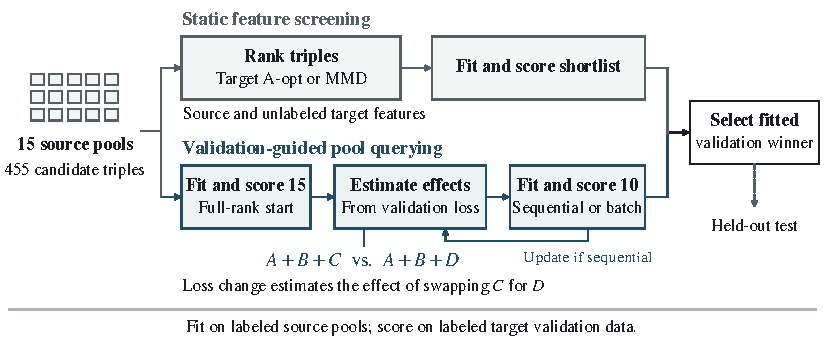
\includegraphics[width=\linewidth]{pool_query_framework.pdf}
\caption{Static screening fixes a shortlist before fitting. At a budget of 25, pool querying fits 15 triples chosen by membership pivots, then uses predicted loss and leverage to choose the remaining ten. The feedback arrow applies to sequential queries. Both routes choose the best validation model among all models they fit before testing.}
\label{fig:pool-query-framework}
\end{figure}

We use this overlap to allocate the remaining fits and compare the resulting policy with screening based on a fixed ranking.

\begin{enumerate}
\interlinepenalty=10000 % Keep each contribution intact across page breaks.
\item \textbf{Choosing later fits from validation feedback.} We fit an initial set of combinations with linearly independent membership vectors and estimate additive pool effects from the observed losses. We score untried combinations by predicted loss and how well earlier fits cover them. We query one at a time or in a second batch and keep the model with the lowest observed loss. Under exact additivity and exact observations, 15 independent queries identify the losses of all triples from 15 pools.

\item \textbf{Explaining what geometric screening captures.} We link Target A-opt to prediction risk in a shared Bayesian linear model and show that closer moment matching can raise risk at equal sample cost. We distinguish screening omissions from selection error within the shortlist.

\item \textbf{Evaluating selection under a fitting budget.} We compare querying with fixed rankings, matched-budget linear designs, and full validation on DomainNet and Optdigits. We hold initial fits fixed to isolate the effect of feedback, repartition the same examples to probe the additive model, and time selection in independent runs.
\end{enumerate}

\section{Related Work}
\label{sec:related}
\subsection{Target-aware experimental design}
A-optimal design measures parameter uncertainty through a covariance trace \citep{fontaine2021}. Transductive design instead weights prediction variance by target covariates \citep{yu2006}. ITL and VTL distinguish where observations can be acquired from where predictions are needed, selecting observations to reduce target entropy or total variance \citep{hubotter2024transductive}. SIFT applies conditional uncertainty reduction to prompt-specific fine-tuning, accounting for redundancy among retrieved examples \citep{hubotter2025sift}. Target A-opt follows the target-variance principle, but ranks fixed pool unions for subsequent supervised evaluation. Separate labeled validation then chooses among the retained combinations.

\subsection{Moment matching and data selection}
MMD compares distribution mean embeddings \citep{gretton2012}; a homogeneous quadratic kernel compares second moments. Moment alignment also supports multi-source domain adaptation \citep{peng2019}. SkMM sketches model gradients to control low-rank approximation bias, then matches moments to control variance during fine-tuning \citep{dong2024skmm}. Related high-dimensional analysis establishes covariance-matching optimality in specific synthetic-data augmentation regimes \citep{rezaei2026synthetic}. Our MMD comparator matches uncentered frozen-feature moments, rather than inheriting those guarantees.

TSDS optimizes a sampling distribution using transport-based target alignment and density-aware regularization against near-duplicates \citep{liu2024tsds}. TAROT instead whitens loss-gradient features before transport-based selection \citep{feng2025tarot}. These methods construct training subsets or sampling weights. We hold candidate membership fixed and compare uncertainty weighting with direct moment matching as ways to reduce supervised evaluations.

\subsection{Geometry and computation budgets}
RankMe assesses representations through effective rank without downstream labels \citep{garrido2023rankme}, and determinantal point processes favor complementary subsets \citep{kulesza2012}. They motivate target-blind comparators. Compute-constrained selection charges scoring against the same budget as training \citep{yin2025}: a better subset need not justify its selection cost. We apply this accounting principle to evaluating pool combinations, measuring both final quality and the work needed to obtain it.

Linear best-arm identification and experimental design use known candidate features to allocate evaluations \citep{soare2014linbai,fiez2019transductive,xu2018lingape,yangtan2022linbai}. Here the candidate features are pool indicators, and observing an arm requires fitting a readout and scoring it on shared validation data. The resulting scores are deterministic under the fixed protocol and can depart from the linear model. Full-bandit combinatorial methods instead model the observed reward as a noisy sum of component rewards \citep{rejwan2020full}. We evaluate how well the linear approximation supports model selection, including designs that reserve a fit to train their predicted recommendation.

\section{Data-Pool Selection}
\label{sec:problem}
\label{sec:theory}
\subsection{Problem and complete procedure}
A pool is a fixed block of examples; a candidate $S\in\cC$ is a feasible union of blocks. The shortlist contains combinations, not individual images. A fixed feature map $h$ comprises the frozen encoder and shared label-independent preprocessing. Let $H_i\in\R^{n_i\times d}$ contain pool $i$'s features, and let $H_S,y_S$ stack the features and labels in $S$. All candidates share a readout fitting rule $\mathcal A$ and a validation loss $L$, fixed before selection.

The static screen uses source features and an unlabeled target-selection set $T_{\rm sel}$ to freeze its shortlist. Each retained candidate fits on source labels and is scored on the separate target-validation set $T_{\rm val}$. Algorithm~\ref{alg:target-a} uses $P_0^{-1}=I$, $\sigma^2=1$ and breaks ties lexicographically.

\subsection{Pool querying with validation feedback}
\label{sec:pool-query}
A query fits a readout on labeled source data from $S$ and returns its Brier loss $v(S)$ on the target validation set. Let $x_S\in\{0,1\}^p$ indicate which of the $p$ pools belong to $S$. Overlap lets us predict validation loss using one effect per pool
\begin{equation}
 v(S)=x_S^\top\beta+r(S),
 \label{eq:pool-additive}
\end{equation}
Here $\beta$ gives the pool effects and $r(S)$ captures departures from additivity.

\noindent\textbf{Choose the first 15 combinations.}
Stack the rows $x_S^\top$ in $X$. Before observing losses, use pivoted Gram--Schmidt to pick the row farthest from the span of selected rows at each step. With alphabetical pool IDs, $\mathrm{ABC}$ comes first and $\mathrm{DEF}$ is the first disjoint triple. The full design has rank 15, so 15 pivots give a unique least-squares estimate. At lower rank, the same queried losses can yield different predictions for untried combinations. Under exact additivity and exact observations, the 15 scores determine all 455 losses (Proposition~\ref{prop:pool-identification}).

\noindent\textbf{Use each new score to choose the next fit.}
For queried rows $Q$, fit $\widehat\beta$ by least squares on $X_Q$ and the observed losses $v_Q$. Choose the unqueried $S$ with the smallest score
\begin{equation}
 x_S^\top\widehat\beta-0.001\sqrt{x_S^\top(X_Q^\top X_Q)^{-1}x_S}.
 \label{eq:pool-acquisition}
\end{equation}
The first term predicts loss. Leverage rewards directions poorly covered by $X_Q$. Fit and score the chosen candidate, then add its row and loss before rescoring. Ten iterations give 25 fits in total. The two-batch variant picks all ten from the ranking computed after the first 15 fits. Both keep the fitted model with lowest observed validation loss (Figure~\ref{fig:pool-query-framework}, Algorithm~\ref{alg:pool-query}).

\subsection{Why target-weighted uncertainty guides screening}
Uncertainty here concerns how feature changes affect predictions, not image clarity or disorder. We formalize it through scalar Bayesian regression with $\theta\sim N(0,P_0)$, $P_0\succ0$, and $y=h^\top\theta+\epsilon$, where independent noise satisfies $\epsilon\sim N(0,\sigma^2)$ and $\sigma^2>0$. Sources and target share $\theta$ and the noise model; target covariates reveal no further information about $\theta$. With target second moment $C_T=\E_T[hh^\top]$, the posterior covariance and posterior-mean target risk conditional on the source design are
\begin{equation}
 P_S=\left(P_0^{-1}+\sigma^{-2}G_S\right)^{-1},\qquad
 R_T(S)=\sigma^2+\tr(C_TP_S).
 \label{eq:risk}
\end{equation}
The risk is irreducible noise plus target-weighted parameter uncertainty, averaging the posterior and a new target observation. Appendix~\ref{app:proofs} gives the derivation.

The score $f_A(S)=\tr(\widehat C_TP_S)$ estimates the second term using unlabeled target features and is minimized with fixed hyperparameters. With an isotropic prior, it is the regularized target-variance criterion of transductive experimental design \citep{yu2006,hubotter2024transductive}; we retain the recorded name Target A-opt. Adding a positive-semidefinite source Gram cannot increase this score.

For the experimental choice $P_0^{-1}=I$ and $\sigma^2=1$, write $G_S=U\operatorname{diag}(\lambda_j)U^\top$, including zero eigenvalues. Then
\begin{equation}
 f_A(S)=\sum_j\frac{u_j^\top\widehat C_Tu_j}{1+\lambda_j}.
 \label{eq:target-directions}
\end{equation}
The reciprocal denominator is the remaining coefficient uncertainty along $u_j$; the numerator weights it by target feature energy. Source coverage reduces the former, while the latter is not known label importance. Combinations with identical spectra can thus receive different scores through their alignment with the target. The implementation evaluates this eigendecomposition form rather than explicitly forming the inverse in Algorithm~\ref{alg:target-a}.

The shared conditional model supplies the risk interpretation of Target A-opt. Its assumption is substantive: if all features equal $1$, source pools labeled constantly $+1$ and $-1$ produce predictors whose risk ordering reverses between two target worlds with opposite constant labels. The feature geometry is unchanged. In classification, we therefore evaluate the scores using trained ridge-softmax and logistic-regression readouts rather than identify Equation~\eqref{eq:risk} with their losses.

\subsection{Moment matching and spectral comparators}
Second-moment matching asks a different question: how close is the source's average directional energy to the target's? With $n_S=\sum_{i\in S}n_i$, it minimizes
\begin{equation}
 f_M(S)=\norm{G_S/n_S-\widehat C_T}_F^2.
 \label{eq:mmd}
\end{equation}
This is empirical squared MMD with kernel $k(h,h')=(h^\top h')^2$, including diagonal terms. It matches average directional energy rather than weighting posterior uncertainty. Both criteria read the same features, testing whether inverse-covariance weighting adds value beyond direct moment matching.

Effective rank instead summarizes the evenness of singular values without target information \citep{roy2007}. It measures spectral shape rather than sample evidence and is a comparator, not a step in Algorithm~\ref{alg:target-a}. Appendix~\ref{app:proofs} defines it and describes how it is computed from the pooled Gram. These comparisons distinguish source diversity, target moment matching, and target-weighted uncertainty within the same selection procedure.

\paragraph{Equal-cost risk reversal.}
Even exact target moment matching can give higher predictive risk in the shared linear model. For eight unit-norm source rows per candidate, take $G_A=\operatorname{diag}(6,2)$, $G_B=\operatorname{diag}(5,3)$ and $C_T=\operatorname{diag}(3/4,1/4)$. Both Gram traces are eight. Squared MMD prefers $A$ ($0$ versus $1/32$), whereas Target A-opt prefers $B$ ($3/16$ versus $4/21$). Appendix~\ref{app:equal-cost-reversal} gives the construction and risk calculation.

\subsection{Separating retention from final selection}
Screening can discard a good candidate; validation can also fail to choose the best retained one. Let $\ell(S)$ be target risk for a fixed trained predictor and $v(S)$ its validation loss. If $|v(S)-\ell(S)|\leq\varepsilon$ throughout $\cQ_s$, the validation minimizer satisfies
\begin{equation}
 \ell(\widehat S)-\min_{S\in\cC}\ell(S)
 \leq
 \underbrace{\min_{S\in\cQ_s}\ell(S)-\min_{S\in\cC}\ell(S)}_{\text{shortlist omission}}
 +2\varepsilon.
 \label{eq:decomposition}
\end{equation}
Omission compares the best retained risk with the best full-family risk. The validation-selection gap is the risk difference between the chosen and best retained candidates, not the validation loss itself. The deviation condition bounds this gap by $2\varepsilon$. The argument needs no shared linear model (Appendix~\ref{app:proofs}). High recall need not yield a good final choice, nor does low final loss require retaining every top-ten candidate. We audit both gaps on finite test data alongside recall, without estimating a population guarantee.

\subsection{Decision budgets and cost accounting}
The full-search reference trains all candidates and chooses $S_{\mathrm{full}}=\arg\min_{S\in\cC}v(S)$. This is a deployable procedure. The test oracle, in contrast, is the candidate with lowest observed test loss and is used only for auditing. Let $b(S)$ be test Brier, the mean squared distance between predicted class probabilities and the one-hot label; lower is better. We report $b(\widehat S_s)-b(S_{\mathrm{full}})$ and the fraction of repeated tasks exceeding a declared absolute tolerance. The gap can be negative because the validation and test rankings can differ.

With frozen features available, screening costs ranking plus fitting and validating retained candidates. Starting from images adds encoder initialization and feature extraction; target-aware scores also need target-selection features. Screening pays off only if its overhead, including extra feature work, is smaller than the evaluations it replaces. Candidate counts are not elapsed time: the matrix operations used in linear scoring can also comprise a substantial part of fitting ridge readouts.

\section{Evaluation Protocol}
\label{sec:protocol}
The studies were conducted in stages. Synthetic tasks test the risk model; PACS and Office-Home \citep{li2017,venkateswara2017} evaluate direct selection against a prespecified practical-effect threshold, followed by a post-hoc headroom audit. The subsequent DomainNet shortlist configuration was frozen before feature extraction and outcome evaluation. Resampling, projection/readout changes, budget reanalysis, and repartitioning are exploratory follow-ups. Independent timing separately measures the cost of executing the selection procedures. Appendix~\ref{app:protocol} records configurations and result locations.

From the official cleaned DomainNet data \citep{peng2019}, we select 100 class names by a fixed hash rule. Each of six domains contributes disjoint sets of 1,536 target-selection images, 1,024 target-validation images, and 3,072 anchor-pool images from official training data, plus 2,048 official test images. The manifest contains 46,080 images. These roles separate information for screening, final selection, and independent evaluation. Class metadata define the benchmark vocabulary but are hidden from screening.

CLIP ViT-B/32 \citep{radford2021} serves as a frozen construction anchor. Within each domain, its first principal-component scores define low, middle, and high strata, each supplying a block of 512 images. For a given target, we exclude its own blocks and enumerate $\binom{15}{3}=455$ combinations, each with 1,536 source images. ResNet-50 and DINOv2-B/14 provide evaluation features \citep{he2016,oquab2024}. All rules share row normalization, a fixed Rademacher projection to 128 dimensions, and post-projection row normalization. Fixed sample count separates data quantity from combination quality; shared encoders and readout settings keep method comparisons from also changing the prediction model.

Target A-opt uses $P_0^{-1}=I$ and $\sigma^2=1$. Comparators are second-moment MMD, target energy $\tr(\widehat C_TG_S/n_S)$, Bayesian D-opt, merged effective rank, subspace DPP, domain balance, and 20 seeded random rankings. They score the same candidate family. Domain balance additionally reads source-domain identifiers. Kernel definitions and tie rules appear in Appendix~\ref{app:protocol}.

The screen produces nested shortlists of sizes $10,25,50,100,227$, with $227$ designated primary. For the fixed-geometry comparison, U2 independently evaluates each method's primary shortlist using ridge regression with regularization $1$, no intercept, and a fixed softmax temperature. Validation Brier selects the final combination, breaking ties lexicographically. Smaller lists reuse that method's nested evaluations; there is no cross-method cache. The test stage verifies upstream hashes before evaluating every combination to establish an exhaustive audit reference.

The archive expands this setup to four projection seeds and adds fixed-regularization multinomial logistic readouts. It preserves candidate membership and shares fitted models across shortlist audits. The new evaluations separately extract ResNet-50 features and fit on hash and first-principal-component (PC1) partitions, and include Optdigits with constructed pools. They lock each validation-based choice before computing test predictions. Resident-feature timings rerun each policy independently. Appendices~\ref{app:protocol} and \ref{app:fresh-eval} give the data and fit protocols.

We measure how many test top-ten candidates survive screening and how far the validation choice lies from the test oracle $S^*$. Recall measures candidate retention, not classification accuracy; regret measures loss relative to the oracle:
\begin{equation}
 \mathrm{Recall}_{10}(\cQ_s)=\frac{|\cQ_s\cap\mathrm{Top}_{10}(b)|}{10},\qquad
 \mathrm{Regret}(\widehat S)=\frac{b(\widehat S)-b(S^*)}{|b(S^*)|}.
 \label{eq:metrics}
\end{equation}
The original acceptance criteria require at least $50\%$ removal, mean recall of at least $90\%$, and mean normalized regret at most $5\%$. Brier is primary. Follow-up negative log-likelihood (NLL) and classification-error audits use their corresponding validation metric to select candidates, with the metric fixed before test access.

We average encoder results within each dataset--target-domain unit and random rankings within each task. PACS/Office-Home contain eight such units and DomainNet six. Follow-up seeds are also averaged within domains. Original bootstrap intervals resample target units; the test-sample analysis fixes trained models and resamples examples within each target. Seeds, encoders, and overlapping combinations are repeated measurements, not additional independent datasets.

\section{Empirical Findings}
\label{sec:results}
We first ask whether screening preserves final quality and saves computation on DomainNet. Retention then separates screening omissions from validation choices, before domain controls and sensitivity tests examine when the geometry is useful. The shared-model and direct-selection studies assess the assumptions behind geometric screening.

\subsection{Final choices across evaluation budgets}
\label{sec:budget}
In the archived projection reanalysis, evaluating 50 Target A-opt or MMD candidates gives lower logistic test Brier than evaluating 227 random candidates in five of six domain averages. Paired mean differences are $-0.001518$ and $-0.001664$, respectively, with descriptive domain-bootstrap ranges of $[-0.003517,0.000023]$ and $[-0.003720,-0.000119]$. Shared source pools make these comparisons dependent. Relative to exhaustive validation, each 50-fit geometric screen exceeds an absolute Brier gap of $0.005$ in one of 48 repeated tasks. The corresponding rate for random screening at 227 fits is $15.52\%$ after averaging random repeats. These fixed-budget comparisons use the archived fits.

\subsection{Low-budget selection with pool queries}
\label{sec:pool-query-results}
Figure~\ref{fig:pool-query-results} and Table~\ref{tab:fresh-pool-query} report fresh DomainNet logistic fits on frozen ResNet-50 features across six domains, four seeds and two partitions. Sequential 25 matches the full-validation winner in 39 of 48 configurations. No test Brier gap exceeds $+0.005$ using $5.5\%$ of the full fit budget. The four paired seed-mean gaps range from $-0.000077$ to $+0.000057$. Linear-design comparisons reveal queried scores from those fits. The separate archived dual-encoder replays also place sequential 25 close to MMD 50 (Appendix~\ref{app:pool-query}).

\begin{figure}[!t]
\centering
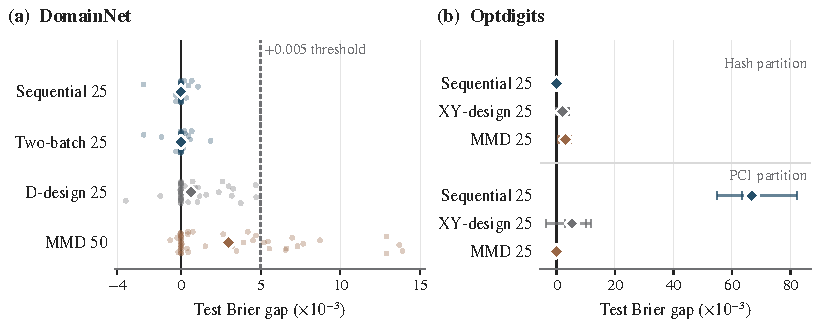
\includegraphics[width=\linewidth]{pool_query_results.pdf}
\caption{Test Brier minus the 455-fit validation-selected reference (solid zero lines). Diamonds show means. (a) Points show 48 DomainNet configurations (six targets, four seeds, two partitions), vertically offset for visibility; the dashed line marks a $+0.005$ descriptive tolerance. (b) For each Optdigits seed the two partitions use the same source examples. Ticks mark four seed results and whiskers span their range. The panels use different horizontal scales. D- and XY-design reserve one of their 25 fits for a predicted recommendation.}
\label{fig:pool-query-results}
\end{figure}

\begin{table}[t]
\centering
\caption{Fresh DomainNet logistic selection. Means weight all 48 configurations equally. SD is across four seed means, each over six domains and two partitions. Gap counts use test Brier minus the full-validation choice. Linear design baselines reserve one of 25 fits for a predicted recommendation. Bold marks the lowest mean at 25 fits.}
\label{tab:fresh-pool-query}
\begin{tabular}{lrrrr}
\toprule
Policy & Fits & Test Brier $\downarrow$ & Seed SD & Gap $>.005$ \\
\midrule
Sequential pool query        & 25  & \textbf{0.916072} & 0.001431 & 0/48 \\
Two-batch pool query         & 25  & 0.916088 & 0.001412 & 0/48 \\
D-design + recommendation    & 25  & 0.916716 & 0.001537 & 0/48 \\
XY-design + recommendation   & 25  & 0.917369 & 0.001446 & 3/48 \\
LinGapE adaptation ($c=.001$) & 25  & 0.916678 & 0.001003 & 3/48 \\
Target A-opt                 & 25  & 0.917241 & 0.001191 & 4/48 \\
MMD                          & 25  & 0.920236 & 0.001685 & 16/48 \\
MMD                          & 50  & 0.919060 & 0.001602 & 13/48 \\
Full validation              & 455 & 0.916078 & 0.001451 & 0/48 \\
\bottomrule
\end{tabular}
\end{table}

Holding the first 15 fits fixed, ten queries guided by the fitted pool effects reduce mean test Brier by $0.003599$ relative to ten additions from the MMD ranking. Dropping the leverage term preserves 47 of 48 sequential winners, and the two-batch variant is within $0.000016$ in mean Brier. The closest linear-design baselines differ by less than $0.001$ in mean test Brier. Appendix~\ref{app:fresh-linear} gives all design baselines, four LinGapE coefficients, and recommendation rules.

Figure~\ref{fig:pool-query-results}b tests the effect of repartitioning the same Optdigits source examples. On hash pools, sequential 25 and full validation both score $0.299730$. On PC1 pools, sequential 25 gives $0.406669$, full validation and MMD 25 give $0.339867$, and XY-design gives $0.345173$. An all-candidate additive fit explains about $85\%$ of the validation-loss variation on hash pools and $17\%$ on PC1 pools. This retrospective diagnostic uses all candidate scores. Under PC1, $169$--$267$ of 455 candidates per seed omit at least one training class. All hash candidates cover all classes. Class coverage and pool interactions may both contribute to the observed gap.

On new DomainNet resident features, the single-worker median is $3.337$ s for sequential 25 and $6.228$ s for MMD 50. With four fitting workers, sequential 25 takes $1.922$ s, two-batch 25 takes $1.154$ s and MMD 50 takes $2.069$ s. For one Clipart configuration timed directly from images once per policy, sequential 25, MMD 50 and full validation take $19.60$, $23.89$ and $76.48$ s. Appendix~\ref{app:fresh-timing} separates these timing settings.

\subsection{Measured decision and feature costs}
\label{sec:cost}
A practical use case is repeated model selection with reusable image embeddings and a small labeled target validation set. Table~\ref{tab:cost} pairs quality and time for static screens at one projection, with independent scoring, fitting, and validation and three runs per encoder--target--readout task.

With projected features in memory, Target A-opt and MMD at size 50 take about one tenth of exhaustive logistic-regression time, with slightly higher Brier than exhaustive validation and lower Brier than random at size 227. Adding measured image-feature work leaves their accounted cost at about $56\%$ of exhaustive validation. Ridge gives nearly identical losses across these choices, but its cheap fits save less than the extra target-selection features cost. The cost reversal identifies when screening overhead matters, despite fewer evaluations. Image totals add measured components, excluding pool construction, downloads, cache serialization, and test auditing. Resident timing excludes disk loading and projection.

\begin{table}[ht]
\centering
\caption{Matched final Brier and mean accounted time in seconds are reported for the two readouts. Resident time includes scoring, fitting, and validation from in-memory projected features. Images adds the separately measured feature work for the fixed pool inventory; it is an additive profile, not a complete pipeline replay. All means use the same timed choices.}
\label{tab:cost}
\begin{tabular}{llrrrr}
\toprule
Readout & Screen & Fits & Brier & Resident (s) & Images (s)\\
\midrule
Ridge & Target A-opt & 50 & 0.986655 & 0.53 & 39.59 \\
Ridge & MMD & 50 & 0.986643 & 0.21 & 39.27 \\
Ridge & Random & 227 & 0.986653 & 0.75 & 35.30 \\
Ridge & Full validation & 455 & 0.986639 & 1.48 & 36.03 \\
Logistic & Target A-opt & 50 & 0.863170 & 4.49 & 43.54 \\
Logistic & MMD & 50 & 0.863110 & 4.31 & 43.37 \\
Logistic & Random & 227 & 0.864241 & 21.23 & 55.77 \\
Logistic & Full validation & 455 & 0.862992 & 42.83 & 77.38 \\
\bottomrule
\end{tabular}

\end{table}

\paragraph{Ridge calibration and fixed-pool transport.}
For the fixed ridge full-validation winners, fitting a temperature on target validation reduces test Brier from $0.986695$ to $0.743338$ at unchanged $36.00\%$ accuracy. Uniform prediction gives $0.99$. With separate validation halves for calibration and reselection, the 50-fit Brier gaps to calibrated full validation are $-0.000150$ for Target A-opt, $+0.002461$ for MMD, and $+0.016541$ for random (Appendix Table~\ref{tab:ridge-calibration}). From resident features and precomputed rankings, either 50-fit screen takes $1.114$ s to fit, calibrate and select, versus $10.047$ s for full validation (Appendix~\ref{app:server-timing}). In the new DomainNet sensitivity study, the calibrated sequential 25-fit policy with fixed regularization exceeds a $+0.005$ gap in 0 of 6 domains at 128 dimensions and 3 of 6 at 256 dimensions. Choosing regularization over three values costs three fits per candidate (Appendix~\ref{app:fresh-ridge}).

On the same 455 candidates with logistic readouts, whitened sliced Wasserstein at 50 fits yields Brier $0.865342$ and takes $0.2948$ seconds to rank candidates from resident features. MMD yields $0.863951$ and takes $0.0387$ seconds. Appendix~\ref{app:calibration-transport} gives both transport variants, the inverse-weighting ablation, and the protocol boundaries.

\subsection{Candidate retention and validation choices}
To distinguish screening omissions from validation choices, Table~\ref{tab:primary} returns to the original DomainNet study. Target A-opt retains nearly all test top-ten candidates while discarding approximately half the combinations. Every primary Target A-opt and MMD shortlist contains a test Brier oracle; remaining regret comes from validation choosing another member. In terms of Equation~\eqref{eq:decomposition}, no empirical oracle omission remains in these lists, but validation selection still affects the final loss.

\begin{table}[t]
\centering
\caption{The fixed-geometry comparison retains $s=227$ of 455 combinations. Means average encoders within six target domains. Recall concerns the test Brier top ten; regret is relative to oracle Brier. Spearman measures agreement between the complete screening and test-loss rankings.}
\label{tab:primary}
\begin{tabular}{lrrr}
\toprule
Screen & Recall (\%) & Regret (\%) & Spearman\\
\midrule
Target A-opt & 98.333 & 0.001311 & 0.7443 \\
Second-moment MMD & 98.333 & 0.001311 & 0.6902 \\
Bayesian D-opt & 82.500 & 0.002658 & 0.4996 \\
Merged effective rank & 81.667 & 0.002909 & 0.4951 \\
Random (20 repeats) & 48.958 & 0.003899 & 0.0016 \\
Target energy & 46.667 & 0.009347 & -0.0399 \\
DPP subspace & 27.500 & 0.009067 & -0.0633 \\
Domain balance & 25.000 & 0.012083 & 0.0681 \\
\bottomrule
\end{tabular}

\end{table}

MMD matches Target A-opt's primary recall and regret and leads validation to the same final combination in every encoder--target task. At smaller budgets, MMD has higher mean recall (Appendix Figure~\ref{fig:recall}). Full-ranking correlation measures agreement across all candidates, whereas recall depends on which good candidates cross the shortlist boundary. Target A-opt's higher correlation therefore need not give better retention. Both outperform the tested target-blind rules here, but the weaker target-energy comparator shows that using target information alone is insufficient: how the score uses it matters.

\subsection{Candidate construction and source-domain controls}
\label{sec:construction}
Does a good shortlist require distinguishing blocks within source domains, or is domain composition enough? We compare mean matching and domain-level moment matching, with projection and readout parameters fixed, on the original blocks and a label- and feature-independent hash partition of the same images. Domain-level matching pools all blocks within each domain before scoring mixtures; it cannot distinguish candidates with identical domain composition. Appendix Table~\ref{app:construction-table} reports this exploratory challenge, separating randomized tie handling from the frozen lexicographic protocol.

Repartitioning preserves the broad Brier advantage over random screening. At size 50, domain-level matching and MMD give similar mean final Brier: domain-level moments suffice for a competitive global shortlist in this setting. Mean matching is competitive on the original blocks but less effective after repartitioning. These comparisons ask whether coarse information suffices overall, not whether blocks within a domain are interchangeable.

The within-composition comparison addresses the latter question. We group candidates containing the same number of blocks from each source domain and retain the floor of half of each non-singleton group. On the original blocks with logistic regression, Target A-opt and MMD retain the empirical Brier optimum in about $77\%$ and $76\%$ of groups, against $45\%$ for random selection. Repartitioning lowers these rates to about $56\%$ and $55\%$; both fall below random for classification error. These are within-group optimum-retention rates, not global top-ten recall. Useful block information can coexist with competitive domain-level matching, but its benefit depends on construction and metric. Neither comparison assigns a causal share of the overall benefit to domain composition.

\subsection{Projection and readout sensitivity}
\label{sec:readout}
Across four archived projections, switching from ridge-softmax to logistic regression increases the relative candidate Brier span from $\RidgeSpan\%$ to $\LogisticSpan\%$. Target A-opt retains $\ReadoutRidgeA\%$ of the test Brier top ten on average with each readout, with MMD slightly higher. At the primary budget, both screens retain a Brier test oracle in every repeated task. Error-based retention reaches as low as $\WorstErrorRecall\%$ for Target A-opt (Appendix~\ref{app:diagnostics}).

\subsection{Target weighting under the shared risk model}
Across 216 synthetic settings, Target A-opt reduces modeled linear risk by $4.23\%$ versus the strongest target-blind effective-rank comparator and $14.85\%$ versus MMD. Descriptive 95\% intervals from resampling settings after averaging seeds are $[3.86,4.62]\%$ and $[13.99,15.70]\%$. In a separate conditional-shift sweep, mean normalized realized prediction regret rises from $0.211$ without shift to $3.143$ at the largest tested shift.

\subsection{Direct selection and available improvement headroom}
PACS and Office-Home test whether the score can directly choose a better source combination. At block budget $K=3$, Target A-opt improves mean within-unit relative Brier by $0.351\%$ over DPP and $0.273\%$ over MMD. Both fall below the prespecified $2\%$ practical-effect threshold. The paired difference interval crosses zero against DPP and is negative against MMD; detailed values are in Appendix~\ref{app:diagnostics}. These comparisons hold block count, rather than source sample count, fixed.
The post-hoc exhaustive audit measures headroom: the loss reduction available from the test-best candidate over the reference. Mean headroom over DPP is only $0.781\%$, limiting average gains without changing the failed prespecified test. This motivates distinguishing better predictions from less evaluation work. These studies provide context, not independent equal-cost screening replications.

\section{Discussion}
\label{sec:discussion}
\subsection{What makes screening useful?}
Screening should be evaluated within the selection procedure. Final loss determines whether fewer evaluations leave an acceptable choice; omission and validation diagnostics explain quality losses. Timing establishes whether work is saved. The readout-dependent cost reversal is central: a useful shortlist need not be economical when fitting is already cheap.
MMD and domain matching show why detailed geometry needs simple matching baselines. Good global choices need not distinguish individual blocks, although block information can help within fixed domain mixtures. Operating points should reflect the target metric, acceptable loss gap, and measured cost together, not recall or full-ranking correlation alone.

\subsection{Limitations}
\label{sec:limitations}
DomainNet targets share source data, and seeds repeat measurements on the same benchmark. Optdigits uses constructed pools. The fixed-budget query results cover 15 pools and 455 candidates; reliable budget selection and detecting additivity failures from a few scores remain open. Query savings reuse the same target validation labels. The $0.005$ gap counts and between-seed variation describe these configurations.

The geometry-derived risk concerns shared linear regression. Shifting label mechanisms, changing the readout, and changing the probability metric can alter empirical classification results. Static image costs add independently measured components; direct pool-query pipeline timing covers a single Clipart configuration. Pool preparation and encoder-pretraining overlap remain outside these tests.

\section{Conclusion}
\label{sec:conclusion}
Pool overlap and validation feedback support low-budget source-combination selection when additive effects predict the loss surface. Fresh DomainNet fits nearly match exhaustive selection in test Brier at 25 fits, and batching cuts elapsed time with parallel workers. Optdigits shows how a different partition can favor geometric screening. The feature costs, readout and loss structure jointly determine the useful operating point.
